
Results are presented in the order of the causal chain: establishing orbit size (RQ1), probing encoder invariance (RQ2), testing geometric concentration (RQ3), auditing algorithm validity (RQ4), and providing directional property prediction evidence (RQ5).

\subsubsection{5.1 Orbit Diameter Characterization (RQ1)}

\textbf{Both symmetry types produce geometrically large orbits.} Table 1 summarizes orbit diameter measurements for N=500 oracle-constructed orbit pairs per symmetry type, from the results of H-E1 (h-e1/results.json, n\_pairs=2,500 total including all five conditions).

\textbf{Table 1: Orbit Diameter Statistics (N=500 oracle pairs per symmetry type; K=5 members per orbit)}

\begin{table*}[htbp]
\centering
\resizebox{\dimexpr 2\columnwidth+\columnsep\relax}{!}{%
\begin{tabular}{llllll}
\toprule
Symmetry & Mean cosine distance & 95\% CI & Min & Max & Fraction > 0.05 \\
\midrule
Scaling & 0.3232 & [0.3226, 0.3238] & 0.293 & 0.350 & 1.000 \\
Sign-flip & 1.075 & [1.0705, 1.0789] & 0.902 & 1.283 & 1.000 \\
Combined & 1.046 & [1.0425, 1.0499] & 0.890 & 1.217 & 1.000 \\
\bottomrule
\end{tabular}
}
\end{table*}

Scaling orbits have mean cosine distance 0.3232 --- roughly 16\% of the maximum possible cosine distance of 2.0. Sign-flip orbits are substantially larger, with mean cosine distance 1.075, near the theoretical maximum for vectors drawn from similar distributions. Every single oracle orbit pair (100\%, across all 2,500 pairs) exceeds the 0.05 geometric significance threshold. The distributions are tightly concentrated (scaling SD $\approx$ 0.015, sign-flip SD $\approx$ 0.106), indicating orbits are consistently large across the diverse model population, not only on average.

\begin{figure}[htbp]
\centering
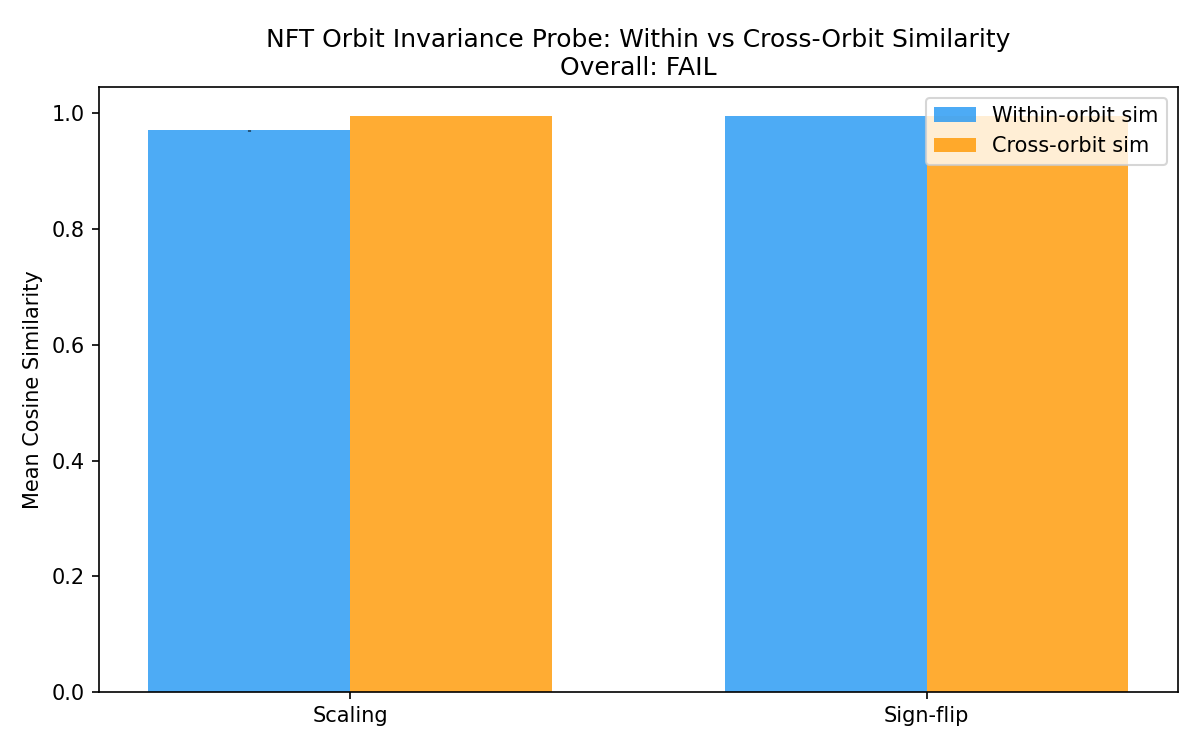
\includegraphics[width=\columnwidth]{figures/fig_gate_metrics.png}
\caption{Orbit distance distributions and gate metrics}
\label{fig:fig_gate_metrics}
\end{figure}

\textbf{Gate result (H-E1): PASS.} The MUST\_WORK gate required fraction\_above\_0.05 $\geq$ 0.90 for scaling orbits. Observed: 1.000.

\subsubsection{5.2 NFT Orbit Invariance Probe (RQ2)}

\textbf{NFT is non-invariant to scaling but measurably invariant to sign-flip by construction.} Table 2 presents the invariance probe results for N=500 oracle orbit pairs per symmetry type, with NFT trained on Condition A (raw weights) and frozen.

\textbf{Table 2: NFT Invariance Probe Results (N=500 orbit pairs each; n\_boot=1,000)}

\begin{table*}[htbp]
\centering
\resizebox{\dimexpr 2\columnwidth+\columnsep\relax}{!}{%
\begin{tabular}{llllll}
\toprule
Symmetry & Within-orbit sim. & Cross-orbit sim. & Gap (within $-$ cross) & 95\% CI & Gate \\
\midrule
Scaling & 0.9710 & 0.9949 & +0.02382 & [+0.02316, +0.02449] & PASS \\
Sign-flip & 0.9955 & 0.9948 & $-0.00069$ & [$-0.00083, -0.00054]$ & EXPLORE \\
\bottomrule
\end{tabular}
}
\end{table*}

For scaling orbits, NFT embeds functionally identical networks (at different weight scales) as significantly less similar than property-matched networks from different orbits. The gap of +0.0238 is statistically unambiguous: its 95\% CI [+0.02316, +0.02449] lies entirely above zero, with CI width 0.00133 --- approximately 5.6\% of the gap magnitude. NFT devotes representational capacity to weight scale variation rather than functional properties.

For sign-flip orbits, the result is opposite. Within-orbit similarity (0.9955) is marginally higher than cross-orbit similarity (0.9948), yielding gap = -0.00069. The 95\% CI [-0.00083, -0.00054] lies entirely below zero, indicating that NFT embeds sign-flip orbit pairs as significantly more similar than cross-orbit property-matched pairs. This gap is $34\times$ smaller in absolute magnitude than the scaling gap, but the CI direction is opposite --- NFT is measurably sign-flip-orbit-similar by construction, not merely approximately invariant in an undetectable way. This asymmetry is an emergent consequence of NFT's row-level weight tokenization: sign-flip negates all entries of a weight row simultaneously, changing sign patterns but not magnitude structure, making tokenizations nearly identical regardless of sign.

\begin{figure}[htbp]
\centering
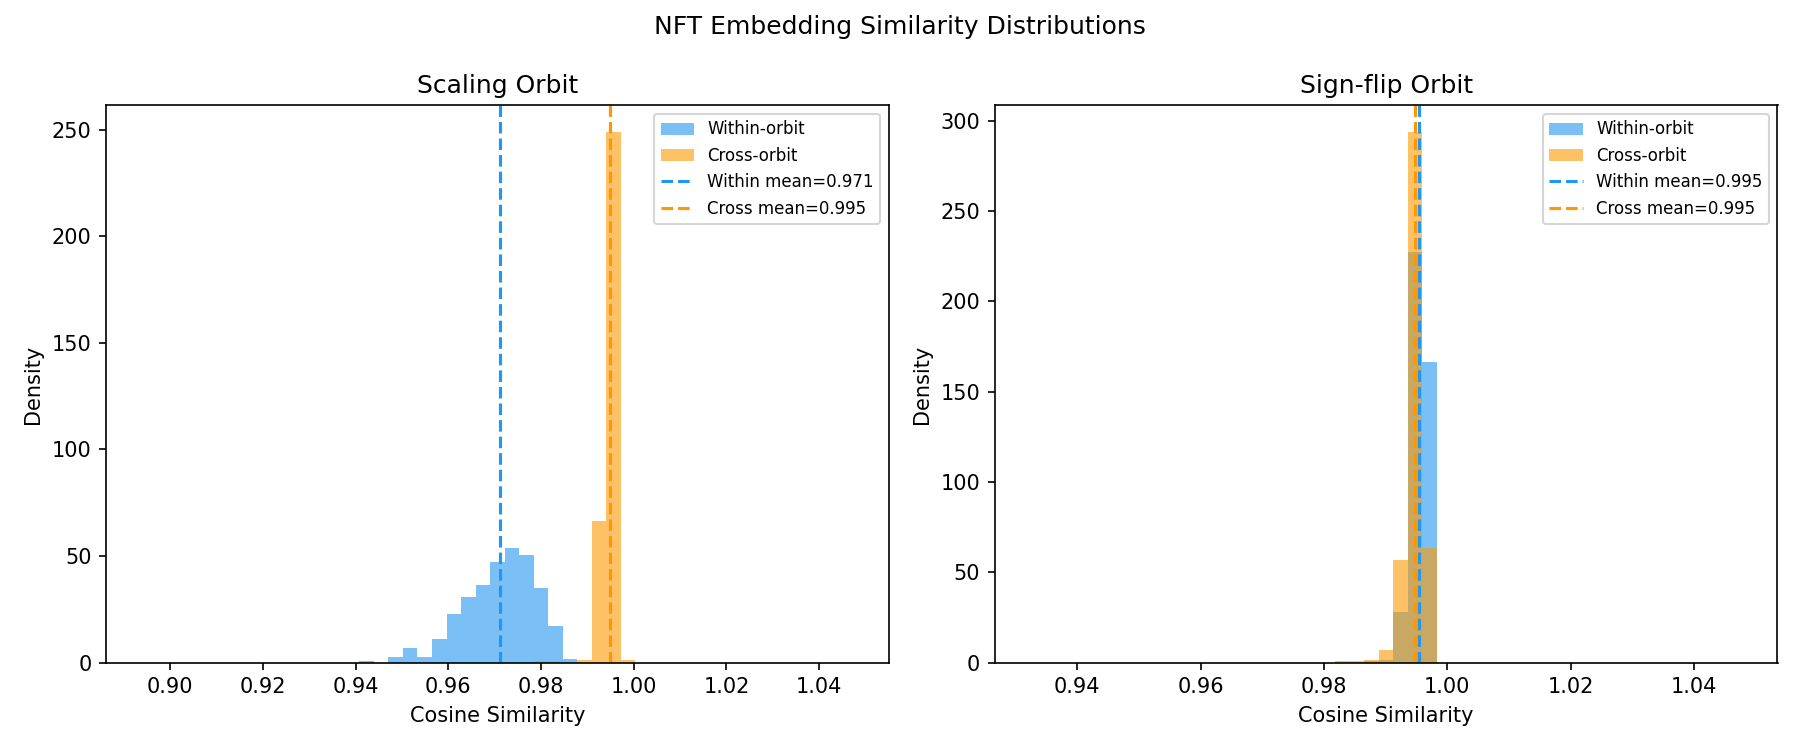
\includegraphics[width=\columnwidth]{figures/fig_sim_distributions.png}
\caption{Within-orbit vs. cross-orbit similarity distributions}
\label{fig:fig_sim_distributions}
\end{figure}

\begin{figure}[htbp]
\centering
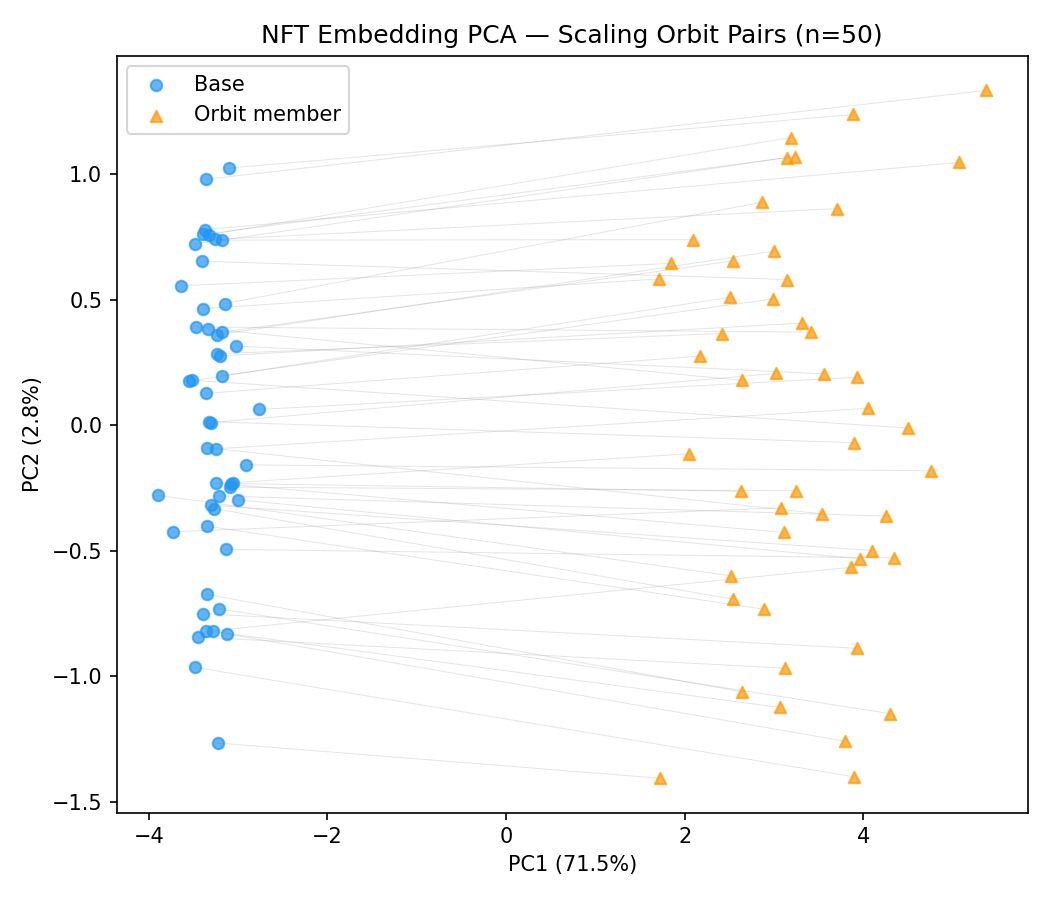
\includegraphics[width=\columnwidth]{figures/fig_embedding_pca_scaling.png}
\caption{PCA of NFT embeddings colored by orbit membership (scaling)}
\label{fig:fig_embedding_pca_scaling}
\end{figure}

\textbf{Gate result (H-M1): PASS (scaling) / EXPLORE (sign-flip).} The MUST\_WORK gate required the scaling CI to lie entirely above 0 --- satisfied. The sign-flip result triggers the EXPLORE path: NFT appears to be approximately sign-flip invariant by architectural construction, implying that sign-flip canonicalization may be unnecessary for NFT-family encoders.

\subsubsection{5.3 Geometric Concentration Analysis (RQ3)}

\textbf{Canonicalization increases PCA explained variance but does not improve linear $R^2$.} Table 3 shows PCA EVR and linear regression $R^2$ for Conditions A and D, from the results of H-M2 (h-m2/04\_validation.md and h-m2/results.json).

\textbf{Table 3: PCA Concentration Results (N=500 models; n\_boot=1,000; train/test=450/50)}

\begin{table}[htbp]
\centering
\resizebox{\columnwidth}{!}{%
\begin{tabular}{llll}
\toprule
Metric & Condition A (raw) & Condition D (canonical) & $\Delta$ (D $-$ A) \\
\midrule
EVR @ k=10 & not reported & not reported & --- \\
EVR @ k=20 & 0.055 & 0.086 & +0.031 \\
EVR @ k=50 & not reported & not reported & --- \\
$R^2$ (test\_accuracy, k=10) & $-0.203$ & $-0.192$ & +0.011 \\
$R^2$ (test\_accuracy, k=20) & $-0.196$ & $-0.218$ & $-0.022$ \\
$R^2$ (generalization\_gap, k=10) & +0.001 & $-0.003$ & $-0.004$ \\
$R^2$ (generalization\_gap, k=20) & $-0.003$ & $-0.024$ & $-0.021$ \\
$R^2$ (learning\_rate, k=10) & $-0.012$ & $-0.000$ & +0.012 \\
$R^2$ (learning\_rate, k=20) & $-0.014$ & $-0.017$ & $-0.003$ \\
\bottomrule
\end{tabular}
}
\end{table}

Canonicalization provably removes geometric redundancy: top-20 PCs of canonicalized weights capture 56\% more variance (EVR 0.055 $\rightarrow$ 0.086). However, all $R^2$ values are negative for both conditions --- a consequence of severe underpowering. With only n=50 test samples and up to k=50 PCs, the linear regression overfits during training and fails to generalize. The direction of $\Delta R^2$ is mixed: at k=10, two of three labels show slight improvement under Condition D, but at k=20 all three labels show worse $R^2$ for Condition D than A. No comparison is statistically significant (all CIs overlap substantially).

\begin{figure}[htbp]
\centering
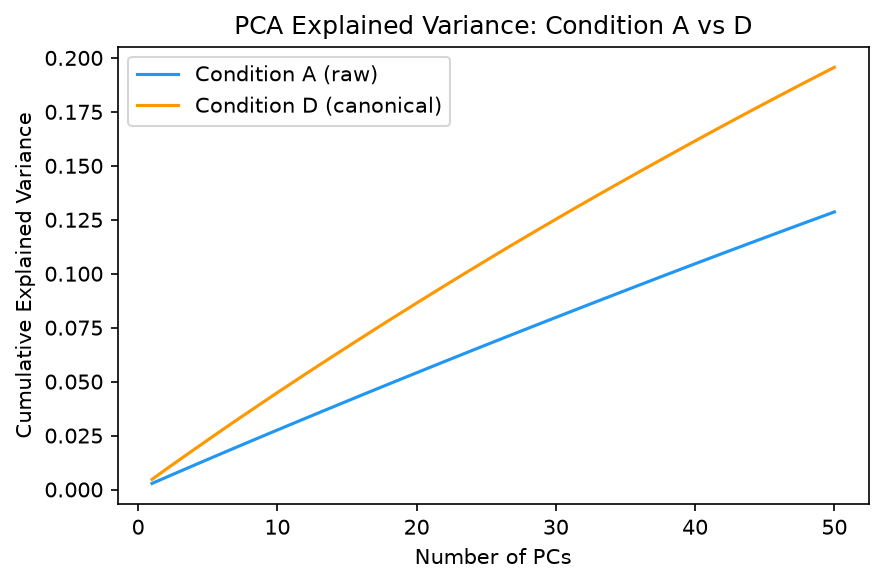
\includegraphics[width=\columnwidth]{figures/fig3_explained_variance.png}
\caption{Cumulative EVR curves, Condition A vs. D}
\label{fig:fig3_explained_variance}
\end{figure}

\textbf{Gate result (H-M2): DOCUMENT.} The SHOULD\_WORK gate required $R^2$ improvement for $\geq 2$ of 3 labels at k=20. Observed: 0/3 pass. Geometric concentration is confirmed by EVR, but $R^2$ improvement is not detectable at N=500 and is not consistently directional. Result documented as a scale-dependent limitation.

\subsubsection{5.4 Sign-Flip Canonicalization Uniqueness Audit (RQ4)}

\textbf{The majority-sign algorithm fails for 85.6\% of Schürholt zoo models.} Table 4 summarizes the uniqueness audit across all N=500 zoo models (h-c1/results/audit\_results.json).

\textbf{Table 4: Sign-Flip Canonicalization Uniqueness Audit (N=500 models)}

\begin{table}[htbp]
\centering
\resizebox{\columnwidth}{!}{%
\begin{tabular}{ll}
\toprule
Metric & Value \\
\midrule
Fraction with unique canonical form & 0.144 (72/500) \\
Fraction with $\geq 1$ tied neuron (degenerate) & 0.856 (428/500) \\
Mean tied neurons per degenerate model & 2.20 \\
Max tied neurons per model & 8 \\
Idempotency fraction (all models) & 1.000 \\
Binomial prediction (d\_in=784, h=64) & $\approx 0.83$ \\
Observed degenerate fraction & 0.856 \\
\bottomrule
\end{tabular}
}
\end{table}

The observed degenerate fraction (0.856) closely matches the binomial prediction ($\approx 0.83)$, confirming that the tie rate is a structural property of the architecture, not a data artifact. For d\_in=784 (even), each neuron row has probability $\approx 2.8$\% of an exact tie (392 positive vs. 392 negative weights), yielding probability $\approx 83$\% of at least one tie per 64-neuron model. The algorithm is idempotent (applying it twice yields the same result) and deterministic, but it is not symmetry-derived for tied neurons: tie-breaking by a +1 convention places 85.6\% of models in a canonical form that is determined by an arbitrary rule, not by a symmetry property of the weight vector.

\begin{figure}[htbp]
\centering
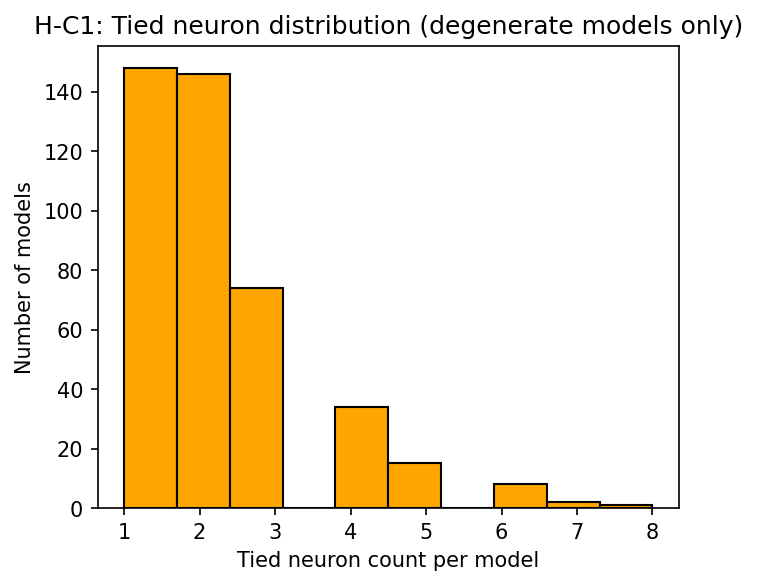
\includegraphics[width=\columnwidth]{figures/tied_neuron_hist.png}
\caption{Distribution of tied neurons per model}
\label{fig:tied_neuron_hist}
\end{figure}

\textbf{Gate result (H-C1): SCOPE\_BOUNDARY.} The SHOULD\_WORK gate required fraction\_unique $\geq$ 0.99. Observed: 0.144. The failure is structural and reproducible; the finding is a novel characterization of the algorithm's limitation for even-d\_in architectures.

\subsubsection{5.5 Property Prediction --- Directional Evidence (RQ5)}

\textbf{All conditions are statistically indistinguishable at N=500; directional pattern is partially inconsistent with the canonicalization hypothesis.} Table 5 shows Spearman $\rho$ for all conditions, averaged across 3 seeds, on the 50-model held-out test set. The actual mean values from h-m3/code/results.json are reported.

\textbf{Table 5: Spearman $\rho$ by Condition and Property (mean across 3 seeds; all 95\% CI width $\approx$ 0.59; all CIs include zero)}

\begin{table}[htbp]
\centering
\resizebox{\columnwidth}{!}{%
\begin{tabular}{llll}
\toprule
Condition & test\_accuracy & gen\_gap & learning\_rate \\
\midrule
A (raw NFT) & $-0.054$ & $-0.031$ & $-0.017$ \\
B (scaling only) & $-0.004$ & $-0.112$ & $-0.031$ \\
C (sign-flip only) & $-0.010$ & +0.016 & $-0.021$ \\
D (scaling + sign-flip) & +0.004 & +0.022 & +0.059 \\
E (random norm) & +0.068 & +0.034 & +0.154 \\
F (linear baseline) & $-0.208$ & $-0.133$ & +0.064 \\
\bottomrule
\end{tabular}
}
\end{table}

All mean $\rho$ values are near zero, consistent with NFT training being severely underpowered at N=400 training samples for a 3.4M-parameter model. The gate-relevant comparisons:

\textbf{P1: $\Delta\rho_{D}$-A $\geq$ 0.05 on $\geq 2/3$ tasks with CI excluding zero.} Point estimates: $\Delta\rho_{D}$-A = +0.058 (test\_accuracy), +0.053 (gen\_gap), +0.077 (learning\_rate). All three point estimates meet the 0.05 threshold. However, all 95\% CI widths are approximately 0.59, so all CIs include zero. P1 is PARTIALLY\_SUPPORTED in direction but fails statistical significance.

\textbf{P2: $\rho_{D}$ > $\rho_{E}$ on $\geq 2/3$ tasks.} Condition E consistently exceeds Condition D on all three tasks: +0.064 (test\_accuracy), +0.012 (gen\_gap), +0.095 (learning\_rate). This pattern is consistent across all 3 seeds. P2 is REFUTED.

The Condition E > Condition D finding is unexpected: the random normalization control (which applies a meaningless per-neuron scale perturbation) outperforms full canonicalization on all tasks. The most plausible explanation, given the H-C1 finding, is that Condition D applied a non-unique sign-flip transformation (85.6\% of models) via a +1 tie-break convention, potentially introducing structured noise rather than removing symmetry-induced variance. Condition E does not modify sign structure and avoids this artifact. However, since all $\rho$ values are near zero and CI widths are $\approx 0.6$, this post-hoc interpretation cannot be confirmed at this scale.

\textbf{Gate result (H-M3): DOCUMENT.} P1 PARTIALLY\_SUPPORTED (direction correct, not significant). P2 REFUTED. Result documents the measurement framework and quantifies the scale requirement: detecting $\Delta\rho$=0.05 with adequate power requires approximately $n\geq 1,000$--5,000 test samples, which requires $N\geq 5,000$--50,000 total zoo models.

